\documentclass[a4paper,9pt]{jsarticle}
\usepackage{stdrep}
\usepackage{url}
\title{ソフトウェアサイエンス実験 S11 最終レポート}
\author{200911434 青木大祐}

\usepackage{amsmath}	% required for `\matrix' (yatex added)
\begin{document}
\maketitle
\newpage

この実験に際して、情報科学類のWebサーバであるwww.coins.tsukuba.ac.jpを用
いて実習を行った。PHPはサーバにインストールされていた5.2.17を、同じく
Perlについてもサーバにインストールされていた5.8.9を使用した。

\section{課題1 WWW上におけるメディア情報検索インターフェイスの作成}
Perlで実装されたサンプルをもとに、PHPを利用して検索エンジンの実装を行っ
た。
\subsection{WWW検索エンジンの作成、データ登録機能の追加}
登録されているデータの表示を行う{\ttfamily index.php}の実装は以下のとお
り。

\lstinputlisting[caption=index.php]{./1-1/index.php}
fgetcsv()関数を使って登録されているデータを読み出し、テーブルとしてペー
ジ内に表示している。\\
\begin{figure}[H]
 \caption{index.php}
 \begin{center}
\fbox{
  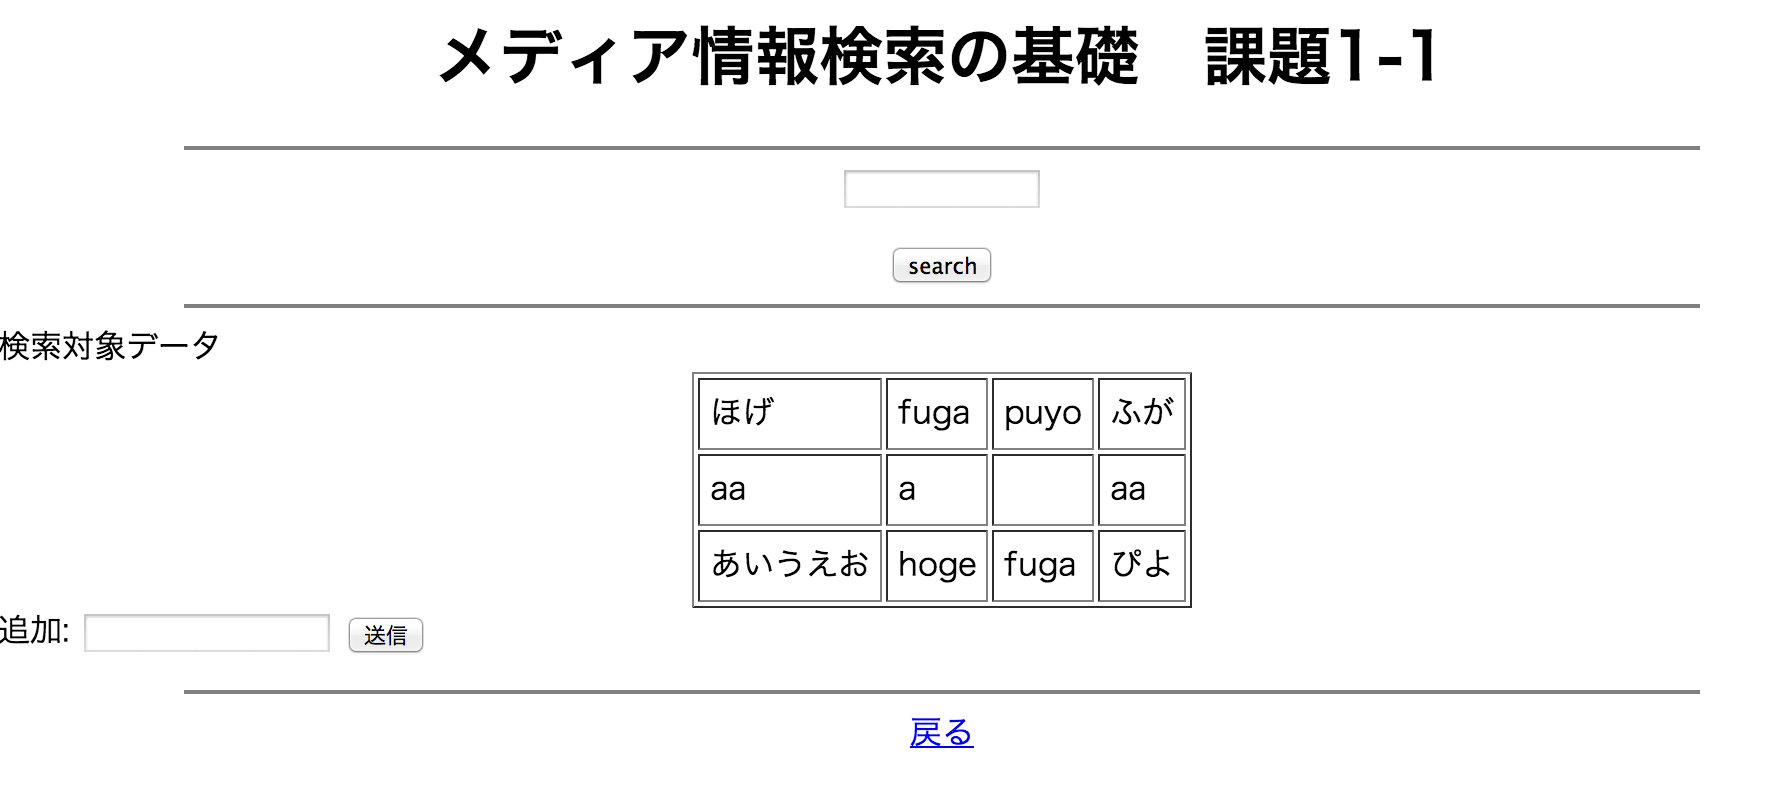
\includegraphics[width=10cm]{fig/1_1_index.png}
}
 \end{center}
\end{figure}

また、データの新規登録には{\ttfamily add.php}を、データの検索には{\ttfamily
search.php}をそれぞれ呼び出している。各部分の実装は以下のとおり。

\lstinputlisting[caption=add.php]{./1-1/add.php}
add.phpでは、与えられたクエリをtarget.txtに書き込み、もとのindex.phpにリ
ダイレクトするという処理を行なっている。

\lstinputlisting[caption=search.php]{./1-1/search.php}
search.phpでは与えられたクエリを登録されているデータの中から探し出し、ヒッ
トしたカラムに色を付けて結果を表示している。

\begin{figure}[H]
 \caption{検索結果}
 \begin{center}
\fbox{
  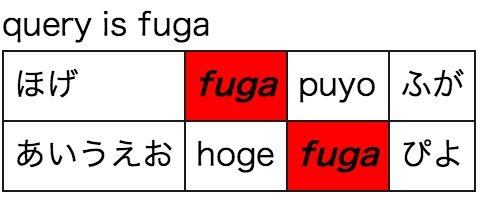
\includegraphics[width=10cm]{fig/1_1_search.png}
}
 \end{center}
\end{figure}
この課題については、
\url{http://www.coins.tsukuba.ac.jp/~s0911434/jikken-s11/1-1/} にアクセスする
ことで実際の動きを確かめることができる。
\section{メディア情報検索システムの構成}
課題2では、検索対象のメディアと類似度の高いものを検索するエンジンを実装
した。
\subsection{類似画像検索システムの実現}
課題2-1では、予め用意されている色情報を用いて類似度の高い画像を検索する
実験を行った。index.phpでは、以下のようにして登録されている画像を列挙し
ている。

\lstinputlisting[caption=index.php]{2/index.php}
このページは以下のように表示される。
\begin{figure}[H]
 \caption{index}
 \begin{center}
\fbox{
  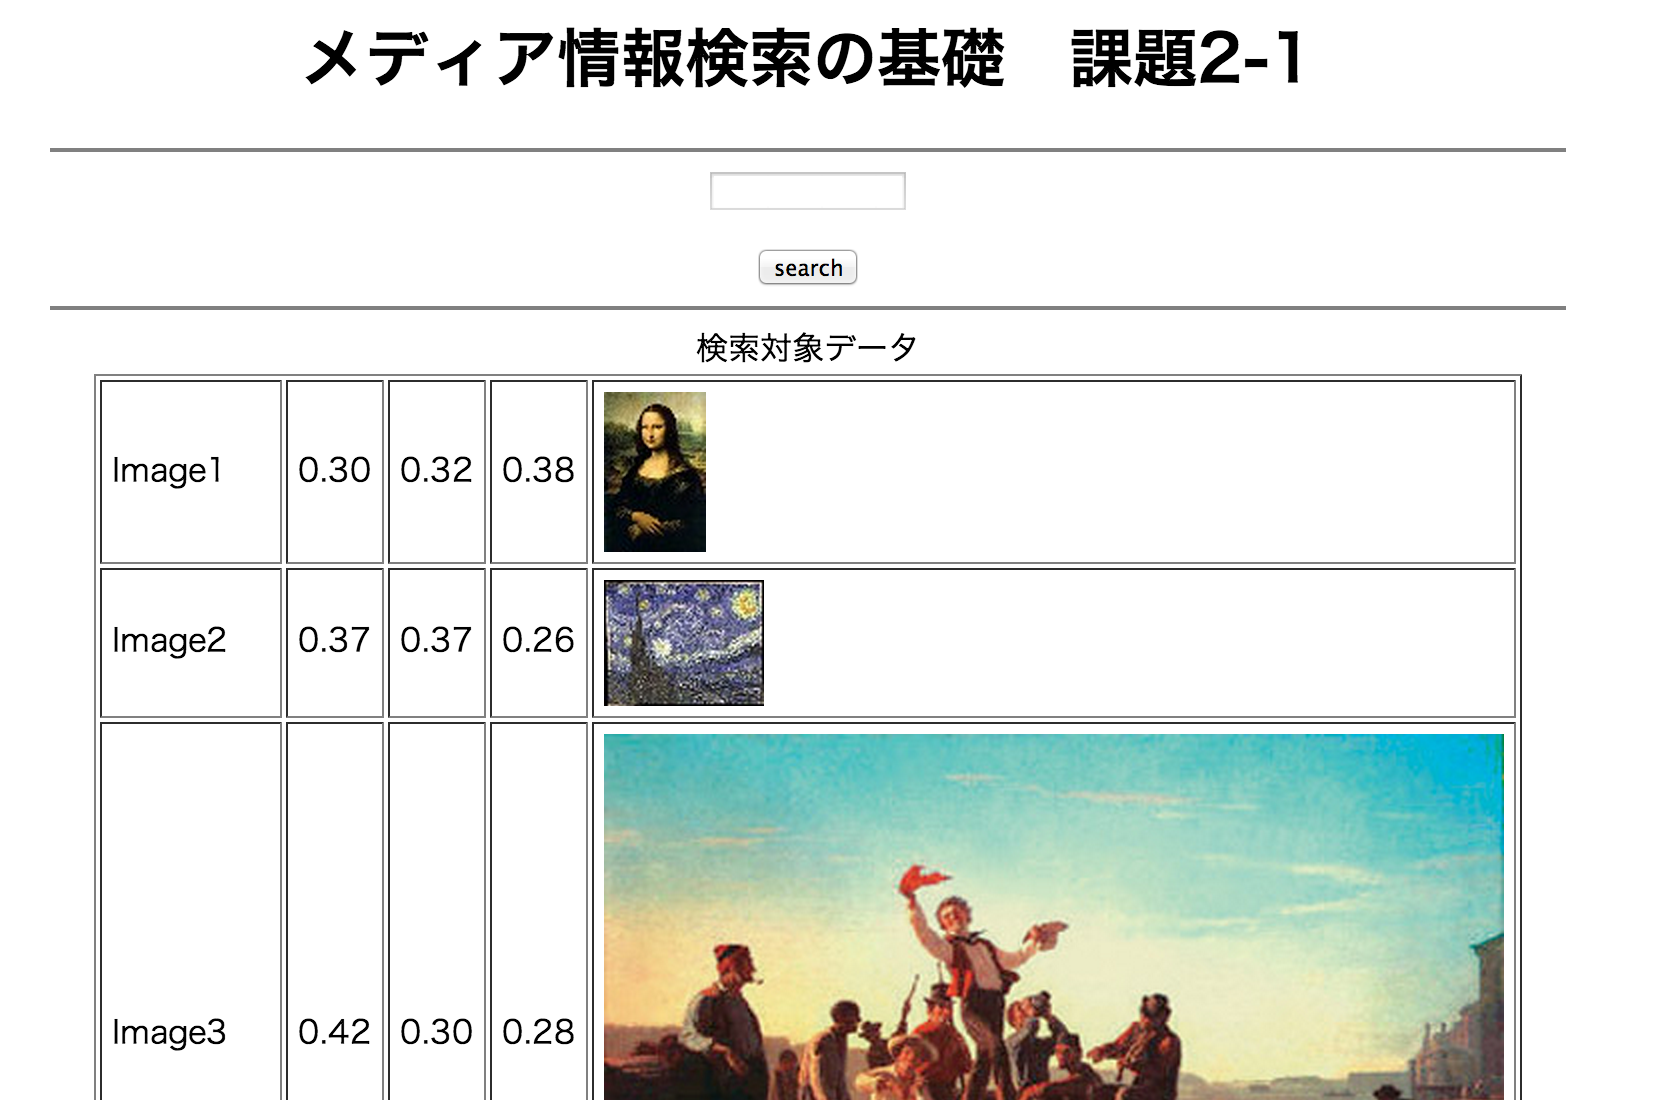
\includegraphics[width=10cm]{fig/2_1_index.png}
}
 \end{center}
\end{figure}
また、ページ下部のフォームからadd.phpにアクセスすることで、任意の画像URLを
追加できる。追加データは「{\itshape 名前, R, G, B, url}」のフォーマット
で記述する。

\lstinputlisting[caption=add.php]{2/add.php}

類似度の計算は、画像の色情報をRGBの三次元ベクトルとして、内積の大きいもの
を類似度が高いと判定している。実際にsearch.phpを用いて類似度の高い順に画
像を並べ替えている。
\begin{figure}[H]
 \caption{検索結果}
 \begin{center}
\fbox{
  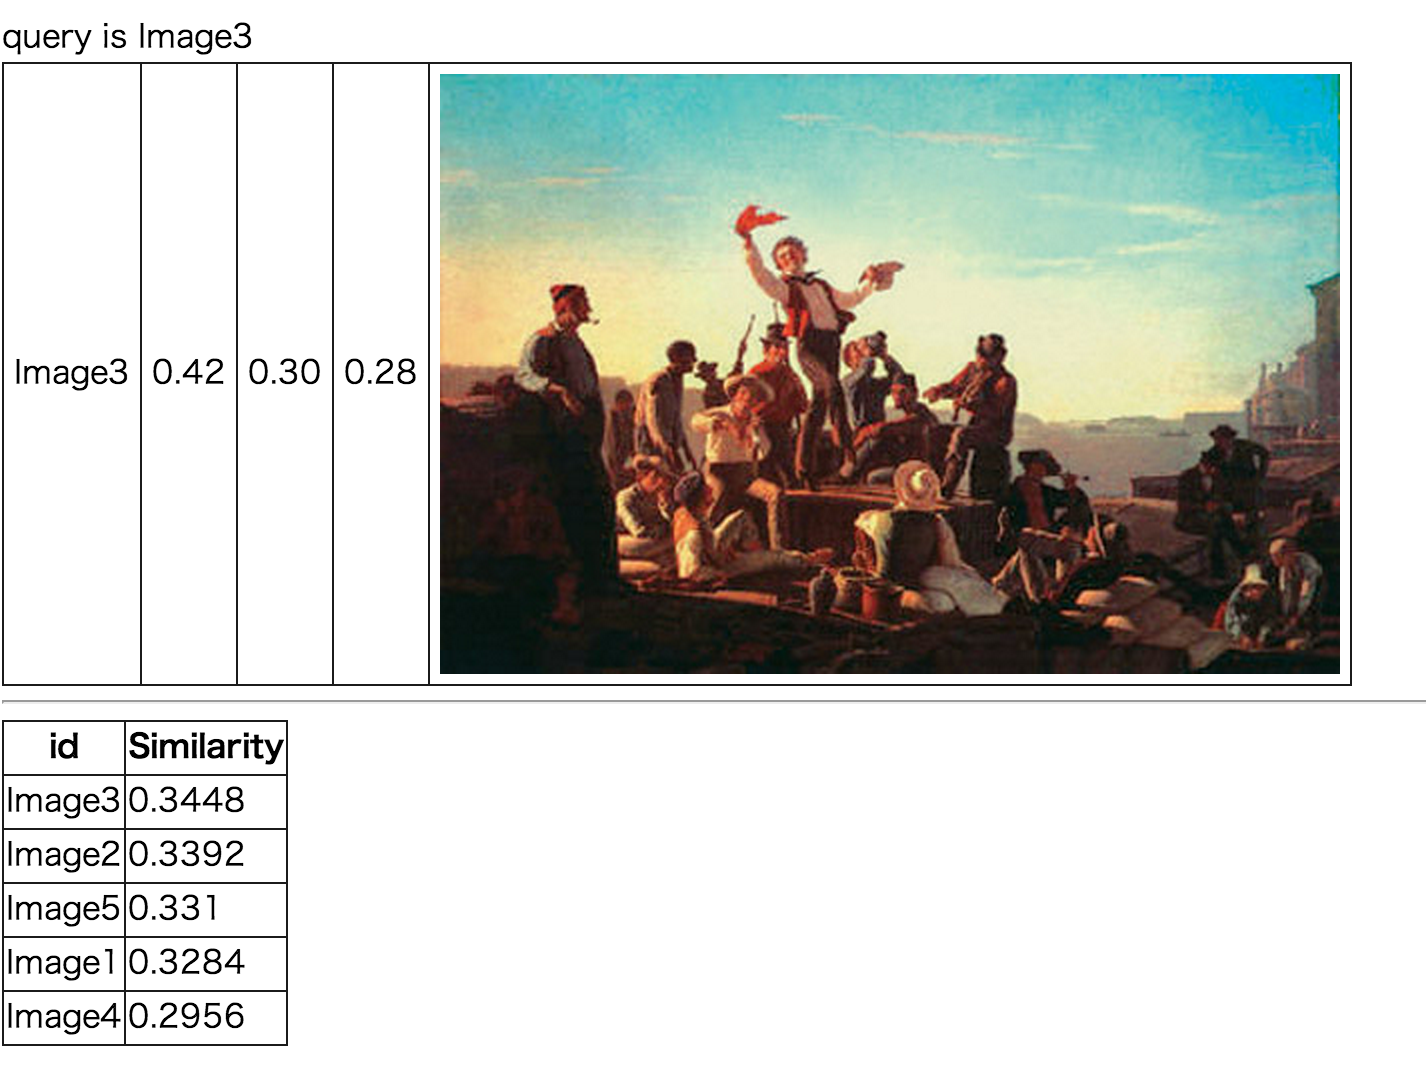
\includegraphics[width=10cm]{fig/2_1_search.png}
}
 \end{center}
\end{figure}

search.phpの実装は以下のとおり。
\lstinputlisting[caption=search.php]{2/search.php}

\subsection{メタデータの自動抽出}
課題2-1において予め用意されていた色情報データを、画像の登録時に自動的に
生成することを考える。add.phpの挙動を変更し、以下の様な処理を追加する。

\begin{enumerate}
 \item 画像のURLを受け取る
 \item wgetコマンドを用いて画像をダウンロードする
 \item ImageMagickのconvertコマンドを用いてppm形式に変換する
 \item ppmファイルを読み込み、色情報データを抽出する
 \item 抽出した色情報データを登録データとして書き込む
\end{enumerate}
以上の操作を行うPerlスクリプトを用意し、add.phpから呼び出すことで、自動的
なメタデータの作成が可能になった。実装は以下のとおり。

\lstinputlisting[caption=add.php]{2-2/add.php}
OSコマンドインジェクション攻撃を回避するため、escapeshellargs関数を用い
て危険な文字をエスケープし、Perlスクリプトに渡している。Perlスクリプトは
検索の際にも用いるため、第二引数としてコマンドの''ADD''を渡し、動作を制
御している。
\lstinputlisting[caption=add\_list.pl]{2-2/add_list.pl}
実際にこのスクリプトが動作するwwwサーバは特殊なディレクトリ構造をしてい
るため、wgetやconvertなどのコマンドパスは決め打ちになっている。

新しく実装したこれらの機能を利用することで、簡単に検索対象となる画像を追
加できるようになった。実際に画像を追加し、indexに反映されているスクリー
ンショットを以下に示す。
\begin{figure}[H]
 \caption{追加された画像}
 \begin{center}
\fbox{
  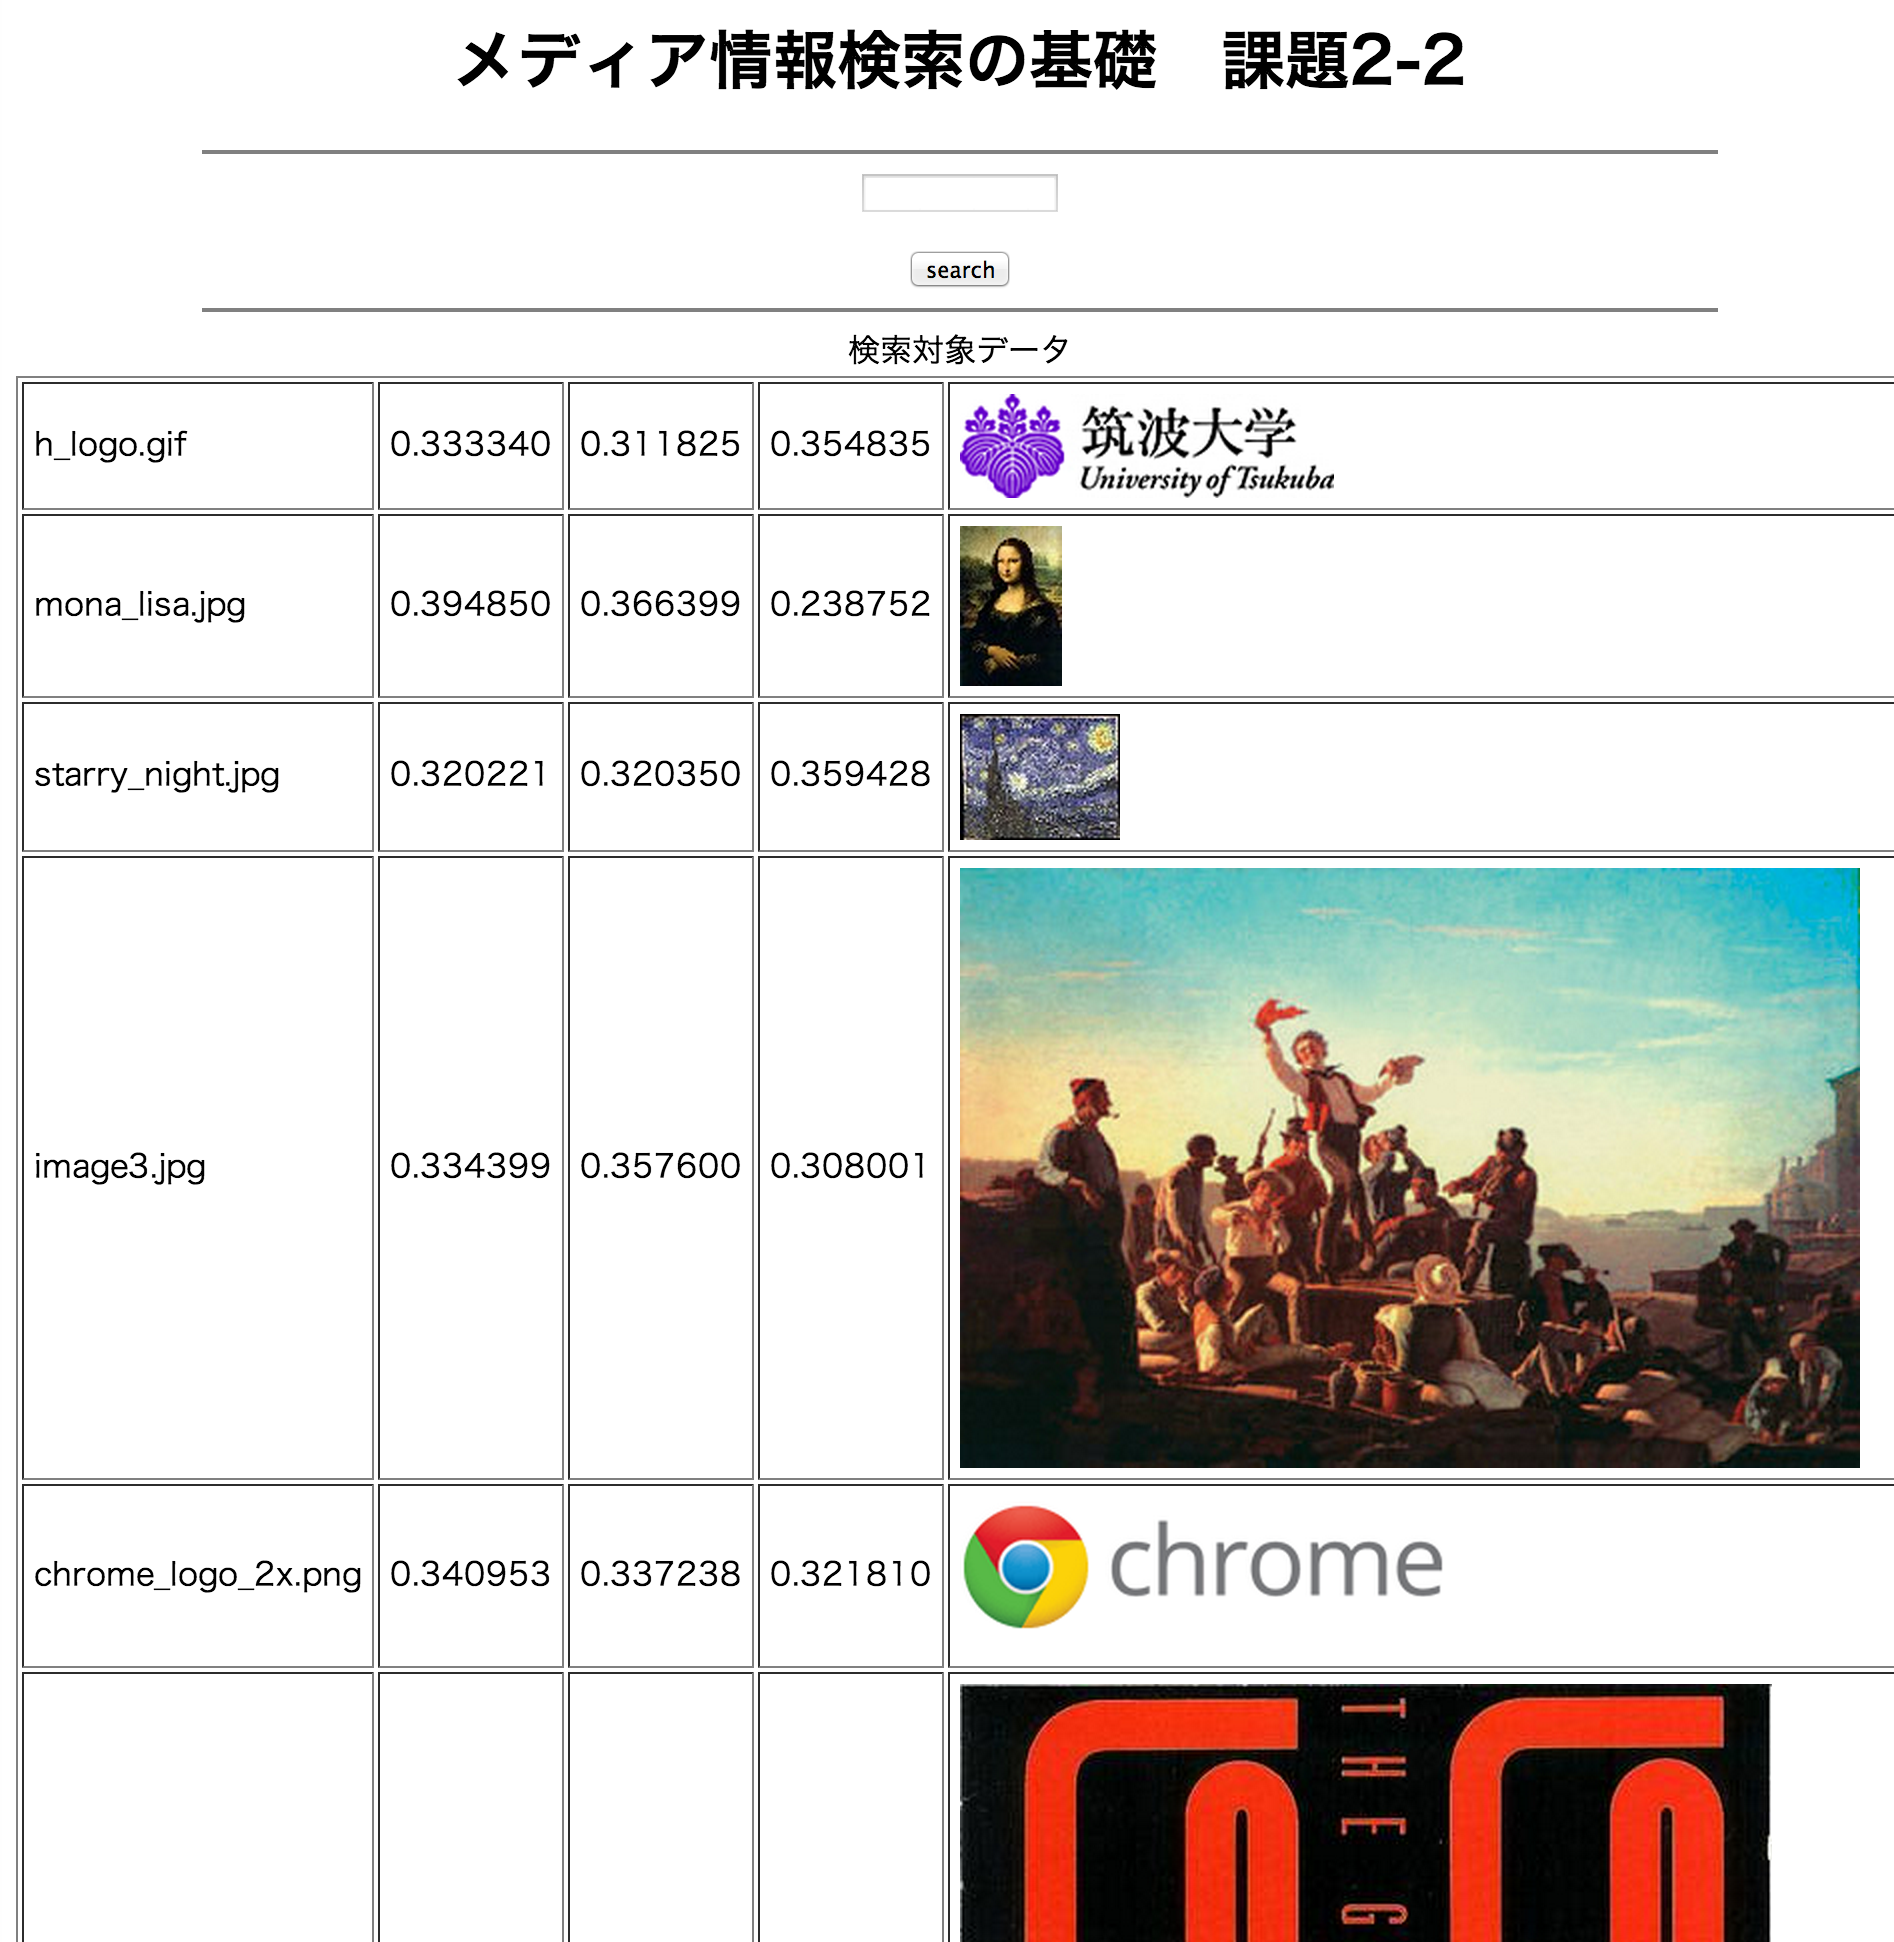
\includegraphics[width=9cm]{fig/2_2_index.png}
}
 \end{center}
\end{figure}
また、search.phpからPerlスクリプトに''SEARCH''コマンドを渡して呼び出すこ
とで、引数に指定したURLの画像から色情報データを抽出し、登録済みの画像か
ら類似度の高いものを表示する事ができる。実際に検索しているスクリーンショッ
トを以下に示す。筑波大学のロゴマークに近い色合いの画像が上位に来ているの
がわかる。

\begin{figure}[H]
 \caption{検索結果}
 \begin{center}
\fbox{
  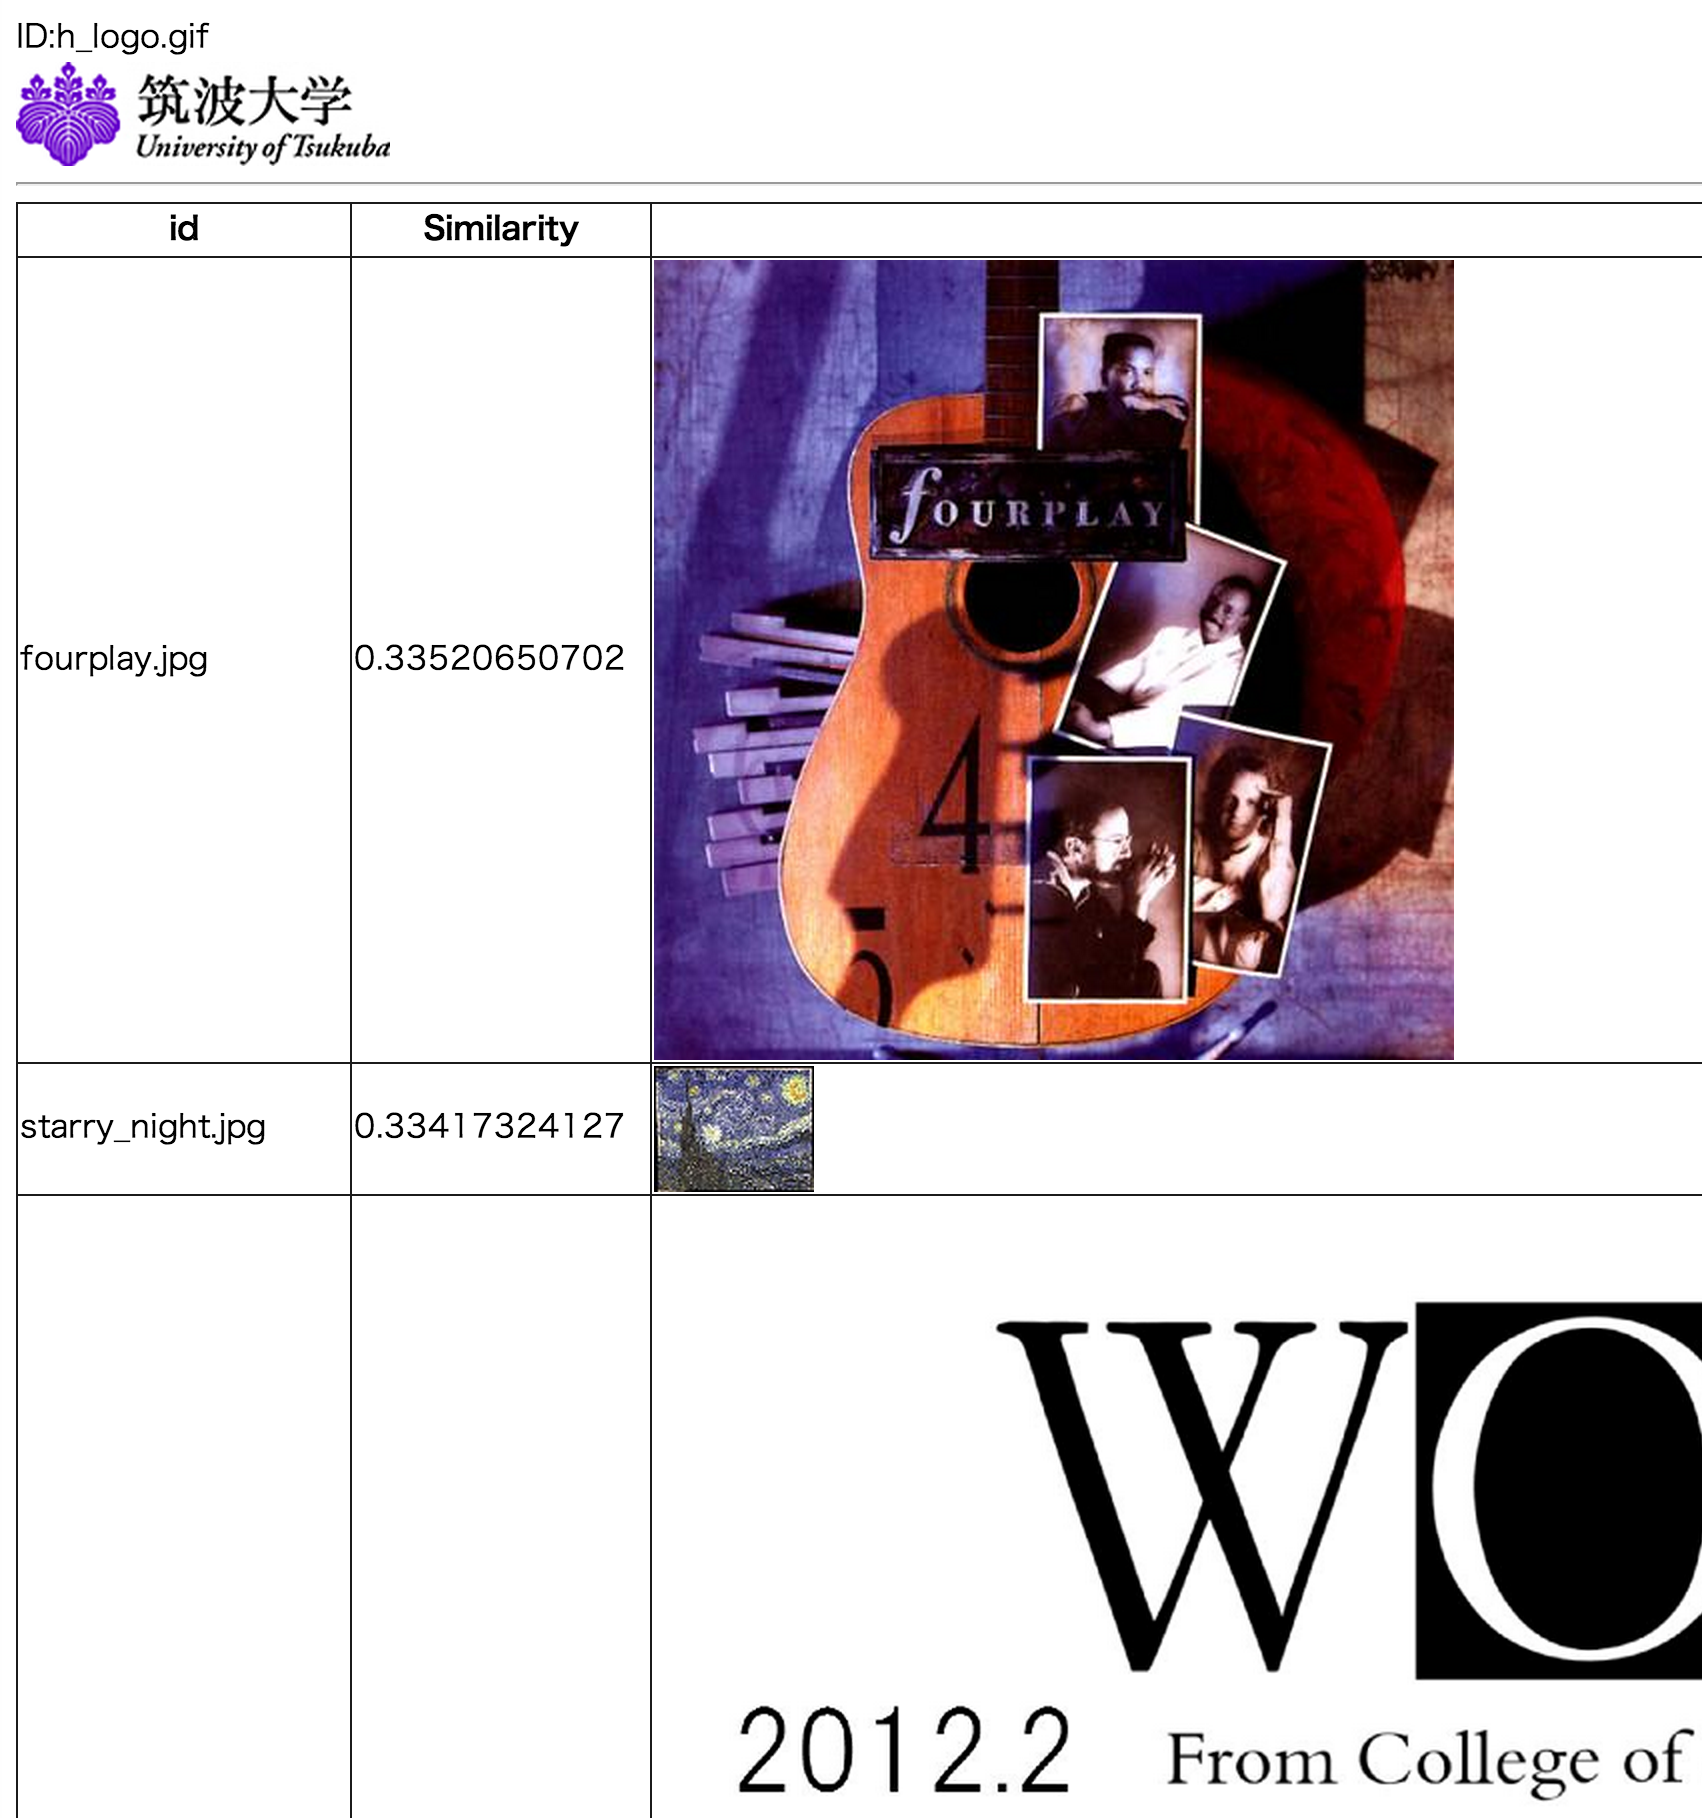
\includegraphics[width=9cm]{fig/2_2_search.png}
}
 \end{center}
\end{figure}

search.phpの実装は以下のとおり。Perlスクリプトから帰ってきた色情報データ
と既存の画像を比較し、類似度の高い順に並び替えて表示している。

\lstinputlisting[caption=search.php]{2-2/search.php}

\url{http://www.coins.tsukuba.ac.jp/~s0911434/jikken-s11/2-2/} にアクセス
することで、これらが実際に機能しているページを触ることが出来る。

\subsection{メディア情報検索システムの実現}
課題2-3では今までとは異なり画像ではないメディアの類似度を計量し、同じ
ように検索を行えるようなシステムを実装した。\\

この課題で対象とするメディアは、英文などローマ字のアルファベットからなるテキスト
ファイルである。単語の出現する頻度をベクトルとして表現し、コサイン類似度を計算
することで、それぞれの文書の傾向から類似度が計算できる。
コサイン類似度の計算については「コサイン尺度(コサイン類似度)の計算
\footnote{http://private.ceek.jp/archives/003891.html}」を参考にし、類似
度の計算部分は同ページに掲載されているサンプルを利用した。\\

また、出現頻度が高く、かつ特徴として意味を成さない助詞や冠詞などの''stop
words''は「Stop Words\footnote{http://www.webconfs.com/stop-words.php}」
のリストを利用し、これらを抽出時に除外した。単語の切り出しや集計などは
Perlで行い、算出したベクトルはテキストファイルとして保存している。\\

英文テキストのコサイン類似度を計算するために実装したPerlスクリプトを以下
に示す。

\lstinputlisting{2-3/add_list.pl}

実際にRFCや日本国憲法の英訳、推理小説、ソースコード、Perl6の仕様書など様々なドキュメントを登録し、
類似度を判定した。\\

無作為に選んだRFCドキュメントを元に類似度順に並べた結果を以下に示す。概
ね登録済みのRFCドキュメントが高い類似度だと判定されている。

\begin{figure}[H]
 \caption{検索結果1:適当に選んだRFC}
 \begin{center}
\fbox{
  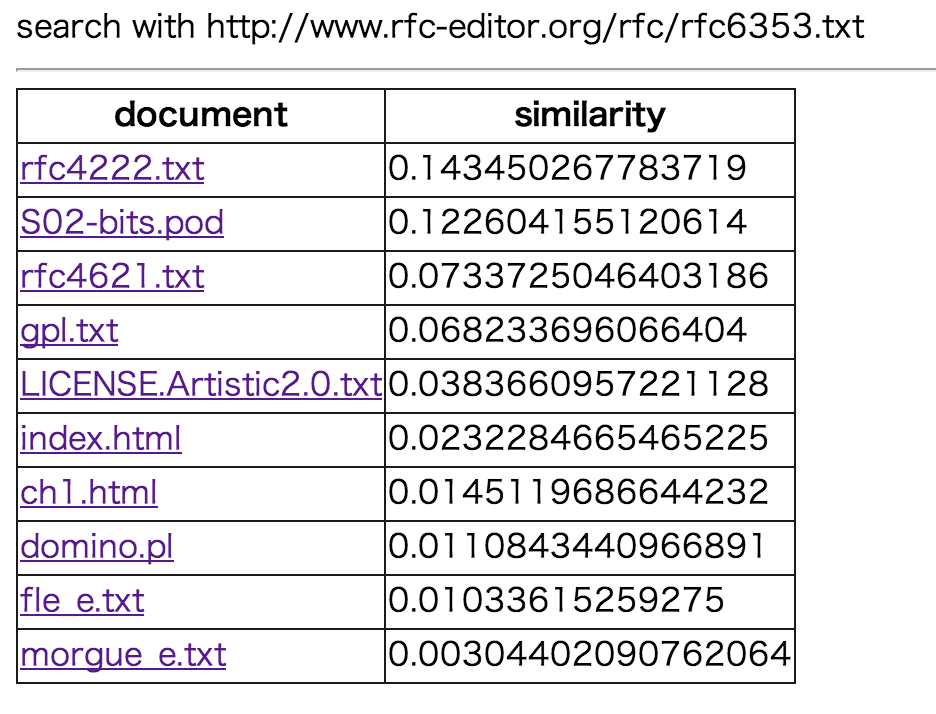
\includegraphics[width=9cm]{fig/2_3_search1.png}
}
 \end{center}
\end{figure}

また、別の例として、登録済みのPerl6の仕様書の別のセクションを与えた場合
の結果を以下に示す。登録済みの仕様書の類似度が非常に高く、また続く2つ目
のソースコードもPerl6で記述されているものである。これらの結果から、この
類似度判定はそれなりの精度を出せていることが分かる。


\begin{figure}[H]
 \caption{検索結果2:仕様書の別セクション}
 \begin{center}
\fbox{
  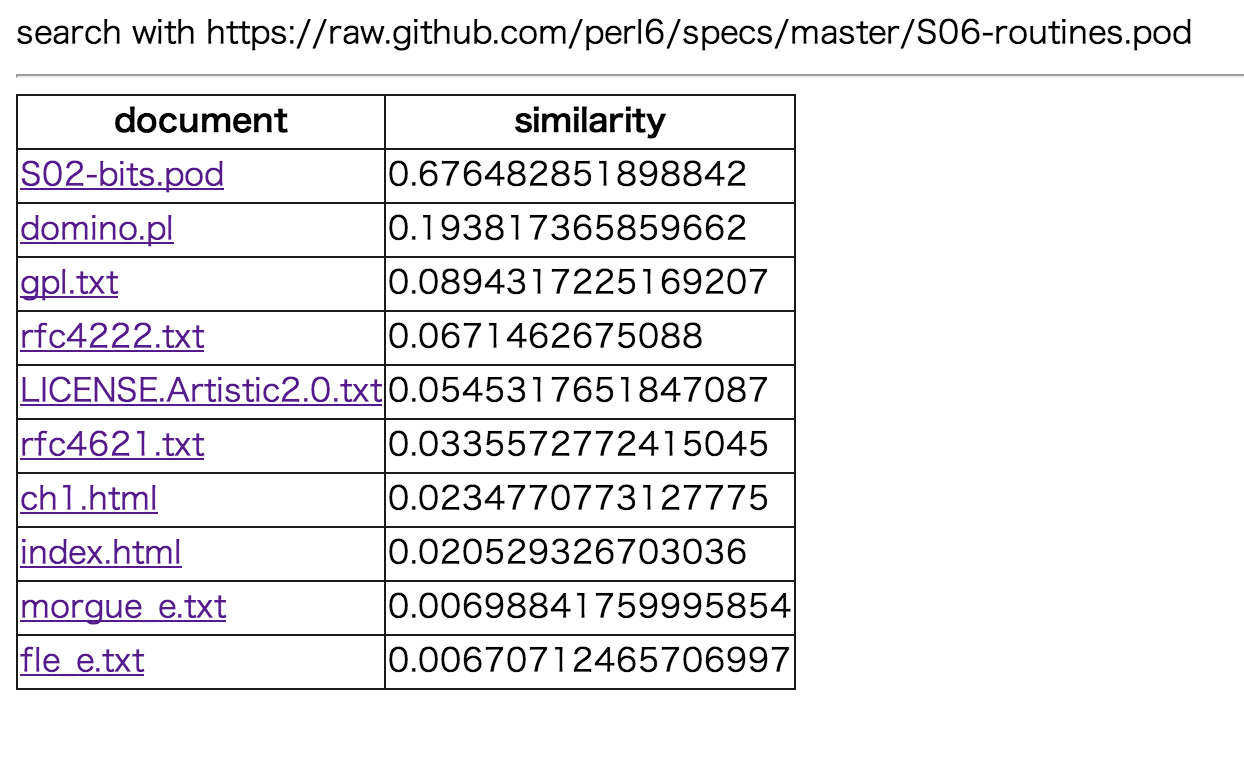
\includegraphics[width=9cm]{fig/2_3_search2.png}
}
 \end{center}
\end{figure}

\url{http://www.coins.tsukuba.ac.jp/~s0911434/jikken-s11/2-3/} にアクセ
スすることで、この類似度判定が実際に動作しているページを触ることが出来る。

\section{メディア情報検索における数理的モデリングの基礎}
課題3では、ページランクに基づく検索結果の重み付けについて実験を行った。

\subsection{PageRankの算出}
ページランクを算出するための仮想的なドキュメントの集合として、次のような
グラフ構造を題材にした。

\begin{equation}
 A=
  \begin{pmatrix}
   0&0&0&1&1&0&1\\
   1&0&0&1&0&1&1\\
   1&1&0&1&0&0&0\\
   1&0&0&0&1&1&0\\
   1&0&0&0&0&0&1\\
   0&1&1&0&1&0&1\\
   1&1&1&0&1&0&0\\
  \end{pmatrix}
\end{equation}

このグラフ構造からページランクを算出するPerlスクリプトを以下に示す。入力
フォーマットは列の先頭にIDとドキュメント名のついたCSVからなるテキストファ
イルである。

\lstinputlisting[caption=pagerank.pl]{3/pagerank.pl}

実行結果として得られたページランクを以下に示す。
\begin{enumerate}
 \item	0.238318
 \item 	0.093458
 \item 	0.070093
 \item 	0.126168
 \item 	0.191589
 \item 	0.065421
 \item 	0.214953
\end{enumerate}

\subsection{PageRankを用いたWeb検索システムの構築}
課題3-1で算出したPageRankを用いて、検索結果の順序を決定するように実装を
行った。検索対象のドキュメントとしては、ある程度同じ単語が含まれるであろ
うRFCを適当に選び、登録を行った。\\

検索の処理を行うsearch.phpの実装を以下に示す。今回はドキュメントの追加な
どは考えないため、ソースコード中にページランクを直接記述してある。
\lstinputlisting{3/search.php}

検索クエリを受け取ると、登録されているドキュメントを順に読み込んでマッチング
を行い、ヒットしたものについては記録しておく。すべてのドキュメントの検索
が終了したら、ヒットしたドキュメントをページランクに基いて並べ直し、検索
結果として表示するという処理を行なっている。\\

実際に検索を行った結果を以下に示す。


\begin{figure}[H]
 \caption{検索結果1:キーワード「RFC」}
 \begin{center}
\fbox{
  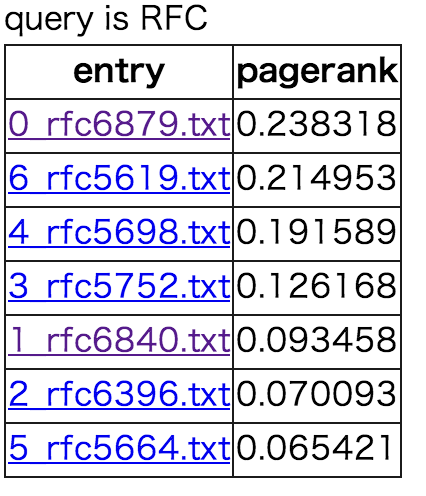
\includegraphics[width=6cm]{fig/3_2_search1.png}
}
 \end{center}
\end{figure}
すべてのドキュメントが検索にヒットしており、検索結果はページランクに基い
て並べられていることが分かる。

\begin{figure}[H]
 \caption{検索結果1:キーワード「algorithm」}
 \begin{center}
\fbox{
  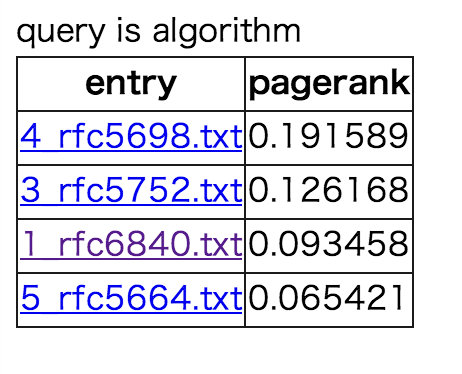
\includegraphics[width=6cm]{fig/3_2_search2.png}
}
 \end{center}
\end{figure}

7つのうち4つのドキュメントに''{\itshape algorithm}''という単語が含まれて
いる。これらもまたページランクに基いて並べられている。\\

以上、ページランクを活用して検索結果を表示する機能が実装できた。このペー
ジは\url{http://www.coins.tsukuba.ac.jp/~s0911434/jikken-s11/3/}にてアク
セスできる。
\newpage

\section{考察}
\subsection{類似度判定について}
抽出方法がまずかったのか、RGBによる内積はあまり精度が高いとは言えない結
果になってしまった。多くの画像は全体的に各色が3.3に近い値をとる傾向にあるため、あまり大きな
差が出なかったのが原因だと考えられる。全体に占める各色の割合だけでなく、
明るさなども計算に入れることで精度をあげられるのではないだろうか。\\
一方、文章のコサイン類似度判定はとてもうまく行ったように思う。語幹の抽出
などは行わずに三単現や過去形などの接尾辞変化などを無視して統計を取ったに
もかかわらず、有意といえる差で類似度が判定できたので満足している。

\subsection{感想}
普段何気なく使っているGoogleなどの検索エンジンであるが、利用者がより簡単
に目的とする情報にたどり着けるように、色々な工夫が成されていることが分かっ
た。単純にリンク数の多いページのページランクが高いということもなく、とて
も良くできた仕組みだということが、実際に実装してみることで実感できたと思
う。

\end{document}
